  %%%%%%%%%%%%%%%%%%%%%%%%%%%%%%%%%%%%%%% -*- coding: utf-8; mode: latex -*- %%
  %
%%%%%                         CHAPTER
 %%%
  %

% $Id: 2200-irure-dolor.tex,v 1.1 2007/11/23 09:52:42 david Exp $
% $Log: 2200-irure-dolor.tex,v $
% Revision 1.1  2007/11/23 09:52:42  david
% *** empty log message ***
%
%

  %%%%%%%%%%%%%%%%%%%%%%%%%%%%%%%%%%%%%%%%%%%%%%%%%%%%%%%%%%%%%%%%%%%%%%%%%%%%%
  %
%%%%%                     HEAD MATTER
 %%%
  %

\chapter{Namespace Locking}
%\addcontentsline{lof}{chapter}{\thechapter\quad Irure Dolor}
%\addcontentsline{lot}{chapter}{\thechapter\quad Irure Dolor}
\label{ch:Locking}

%\begin{quotation}
%  {\small\it Neque porro quisquam est qui dolorem ipsum quia dolor sit amet, consectetur, adipisci velit...}
%
%{\small\it -- Cerico}
%\end{quotation}

\subsection{The Namespace Locking in GFS}

Unlike traditional file systems, GFS doesn't have a per-directory data structure, which means that it doesn't support listing all files in a directory (i.e, \textit{ls} in POSIX), nor aliasing for the same file or directory (i.e, hard or symbolic links). Instead, with prefix compression, GFS represents the namespace as a lookup table mapping full pathnames to metadata logically. Therefore, each node in the namespace tree will be associated a \textit{read-write} lock. To prevent deadlock, locks are acquired in a consistent total order: first ordered by level, then lexicographically within the same level~\cite{ghemawat2003google}.

\noindent One benefit for the locking scheme in GFS is that it allows concurrent mutations within the same directory. 

\begin{figure}[ht]
	\centering
	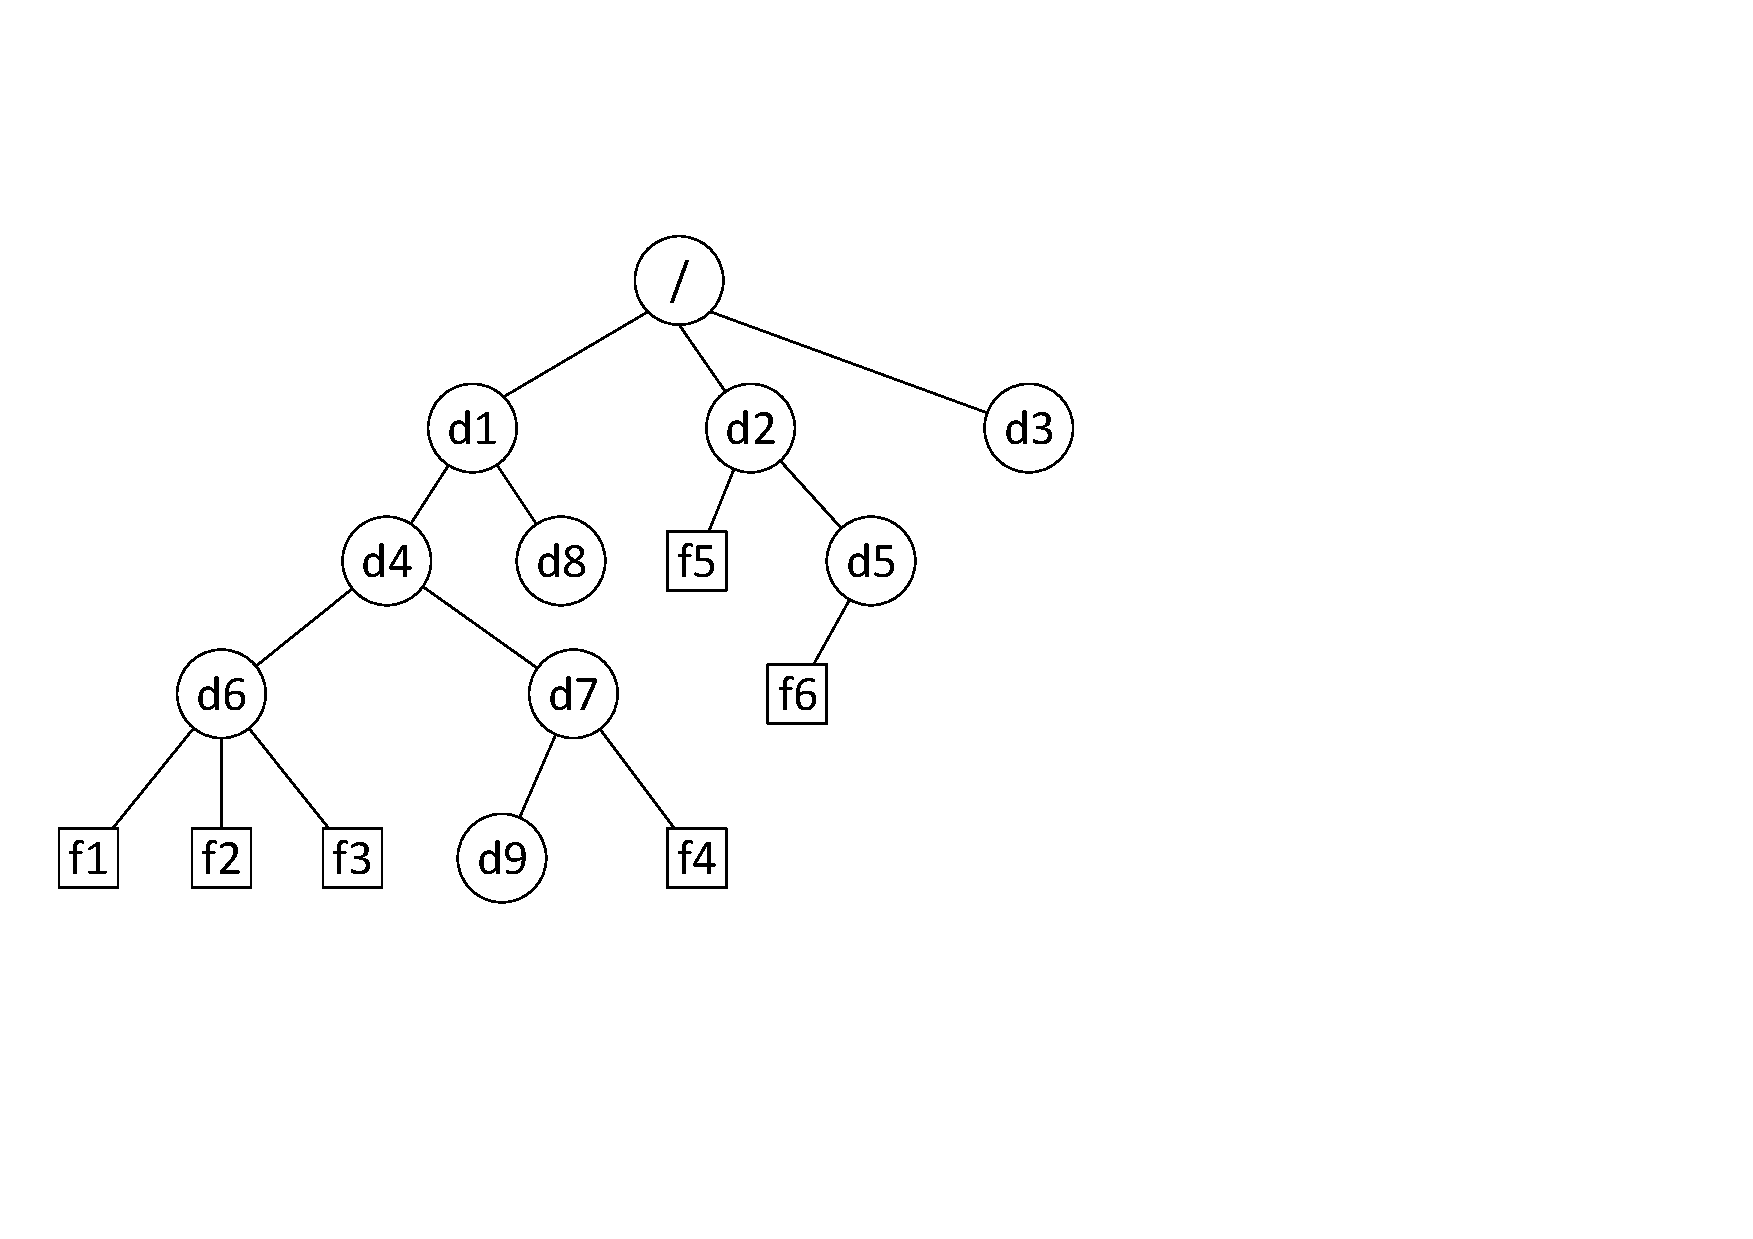
\includegraphics[scale=0.6]{figs/gfstree.pdf}
	\caption{A Graphical Tree Representation for the Namespace in GFS}
	\label{fig:gfsTree}
\end{figure}

\noindent For example, suppose that we have a graphical tree representation for the namespace in GFS as shown in Figure~\ref{fig:gfsTree}. Concurrently, we have five operations involving files \textit{f1, f2, f3, f4} and directory \textit{d9}. These five operations are all allowed.
  %%%%%%%%%%%%%%%%%%%%%%%%%%%%%%%%%%%%%%%%%%%%%%%%%%%%%%%%%%%%%%%%%%%%%%%%%%%%%
  %
%%%%%                        FIRST SECTION
 %%%
  %

\section{A}




  %%%%%%%%%%%%%%%%%%%%%%%%%%%%%%%%%%%%%%%%%%%%%%%%%%%%%%%%%%%%%%%%%%%%%%%%%%%%%
  %
%%%%%                      SECOND SECTION
 %%%
  %

\section{B}


  %%%%%%%%%%%%%%%%%%%%%%%%%%%%%%%%%%%%%%%%%%%%%%%%%%%%%%%%%%%%%%%%%%%%%%%%%%%%%
  %
%%%%%                         ANOTHER SECTION
 %%%
  %
\section{C}

CCC

  %%%%%%%%%%%%%%%%%%%%%%%%%%%%%%%%%%%%%%%%%%%%%%%%%%%%%%%%%%%%%%%%%%%%%%%%%%%%%
  %
%%%%%                          LAST SECTION
 %%%
  %

\section{D}

DDD

  %
 %%%
%%%%%                           THE END
  %
  %%%%%%%%%%%%%%%%%%%%%%%%%%%%%%%%%%%%%%%%%%%%%%%%%%%%%%%%%%%%%%%%%%%%%%%%%%%%%

%%% Local Variables: 
%%% mode: latex
%%% TeX-master: "tese"
%%% End: 
